\documentclass[dvipdfmx]{standalone}
\usepackage{tikz}
\usetikzlibrary{calc}

\begin{document}

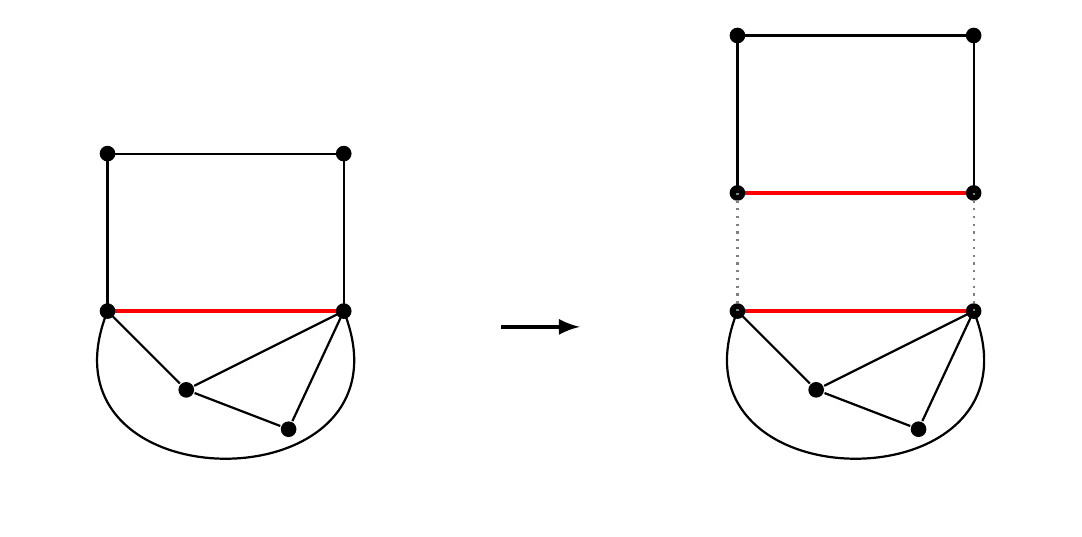
\begin{tikzpicture}[>=latex, thick]
    \tikzset{
        dot/.style={circle, fill=black, inner sep=2pt},
        shared_edge/.style={ultra thick, red}
    }

    \begin{scope}[local bounding box=UnionGraph]
        \coordinate (L_u) at (-1.5, 0);
        \coordinate (L_v) at (1.5, 0);
        \coordinate (L_x) at (1.5, 2);
        \coordinate (L_y) at (-1.5, 2);
        \draw (L_u) .. controls (-2.5, -2.5) and (2.5, -2.5) .. (L_v) -- cycle;
        \node[dot] (g1) at (-0.5, -1) {};
        \node[dot] (g2) at (0.8, -1.5) {};
        \draw (L_u) -- (g1) -- (L_v);
        \draw (g1) -- (g2) -- (L_v);
        \draw (L_u) -- (L_y) -- (L_x) -- (L_v);
        \draw[shared_edge] (L_u) -- (L_v);
        \foreach \p in {L_u, L_v, L_x, L_y} \node[dot] at (\p) {};
    \end{scope}
    \draw[->, ultra thick, shorten >= 1cm, shorten <= 1cm] 
        (UnionGraph.east) -- ++(3, 0);
    \begin{scope}[shift={(8, 0)}, local bounding box=SepGraph]
        \coordinate (R_u) at (-1.5, 0);
        \coordinate (R_v) at (1.5, 0);
        \draw (R_u) .. controls (-2.5, -2.5) and (2.5, -2.5) .. (R_v) -- cycle;
        \node[dot] (rg1) at (-0.5, -1) {};
        \node[dot] (rg2) at (0.8, -1.5) {};
        \draw (R_u) -- (rg1) -- (R_v);
        \draw (rg1) -- (rg2) -- (R_v);
        \draw[shared_edge] (R_u) -- (R_v);
        \foreach \p in {R_u, R_v} \node[dot] at (\p) {};
        \begin{scope}[yshift=1.5cm] 
            \coordinate (R_Hu) at (-1.5, 0);
            \coordinate (R_Hv) at (1.5, 0);
            \coordinate (R_Hx) at (1.5, 2);
            \coordinate (R_Hy) at (-1.5, 2);
            \draw (R_Hu) -- (R_Hy) -- (R_Hx) -- (R_Hv);
            \draw[shared_edge] (R_Hu) -- (R_Hv); 
            \foreach \p in {R_Hu, R_Hv, R_Hx, R_Hy} \node[dot] at (\p) {};
        \end{scope}
        \draw[dotted, gray] (R_u) -- ++(0, 1.5);
        \draw[dotted, gray] (R_v) -- ++(0, 1.5);
    \end{scope}

\end{tikzpicture}

\end{document}